%!TEX root = main.tex

\subsection{Research Thrust 2: Reach-ability analysis based safety region estimation}
\label{sec:reachability}
\nicola{This is all you Nicola}
\lu{Lu adds subsection on control synthesis}

\nicola{The goal of this section is to define a method to quickly assess safety (and perhaps trust) online and then use this reachability analysis to close the loop and correct the system to maintain safety and increase trust}

\nicola{Here discuss recent work on reachability analysis for safety then add the new ideas on online reachability using machine learning and control to predict future states while guaranteeing safety and adapt. }

%%%%%%%%%%%
%%%%%%%%%%%
%%%%%%%%%%%

\paragraph{Approach:} 
\NB{need to improve this section} This thrust is divided in two main parts, as outlined in Figure\NB{add figure}. We start by proposing a reachability-based approach in which we leverage knowledge about the system dynamics and process, sensor, and environmental uncertainties to determine the future states over a finite time horizon. The computed reachable sets will be used to determine the first time that a safety-critical event may occur. 
More specifically, in this work we are interested in the fist time that the AV may: i) collide with any obstacle, both static and dynamics ii) deviate from the desired trajectory, and/or iii) suffer a failure \NB{what do you all think? Can we add somethng related to trust?}. Based on these events, we will then design a safe reinforcement learning approach to adapt and correct the behavior of the system to maintain safety and increase trust \NB{it would be nice to connect trust here}. Here we propose also techniques for fast verification and monitoring \NB{I will elaborate and rephrase}.

%self-triggered scheduling scheme to decide the optimal time to sense and replan. In this way, both energy and computation resources can be minimized to extend the life of the system and better allocate resources to other tasks. We also propose an event-triggered approach to deal with unpredicted sudden events like for example failures or unmodeled disturbances.
%
%To deal with uncertainties in system's model we propose to investigate: i) stochastic reachability analysis which allows us to treat the system as a stochastic hybrid system and ii) reinforcement learning to deal with more complicated changes like system's failures.


\vspace{10pt}
\noindent\textbf{Online Prediction}
%Self-Assessment via Reachability Analysis.}
%\NB{Expectation-Maximization and Hidden markov model}\NB{look at Julia sets maybe for future work} The main question that we are interested to answer here is: What's the likelihood that the system will be able to complete its task without creating safety concerns?

\noindent\textbf{\em Reachability-based Approach:} Traditional model-predictive or finite horizon controllers (MPC) \cite{bernardini2012stabilizing, elnaggar17AHS, bezzo2016stochastic} can estimate future states and inputs of a system, given a correct knowledge of its model. On the other hand, reachability analysis (RA) \cite{TomlinRAM11, TomlinICRA11, esen18} provides regions that can be reached by the system when applying a sequence of inputs and assuming different uncertainties like process noise, model uncertainties, sensor noise and jitter, delays, and external disturbances. For this reason RA is typically used to monitor and assess if and when safety conditions can be violated \cite{gillula2011applications, gillula2010design, althoff2010reachability}.

\begin{wrapfigure}{R}{0.35\linewidth}
\vspace{-5pt}
\centering
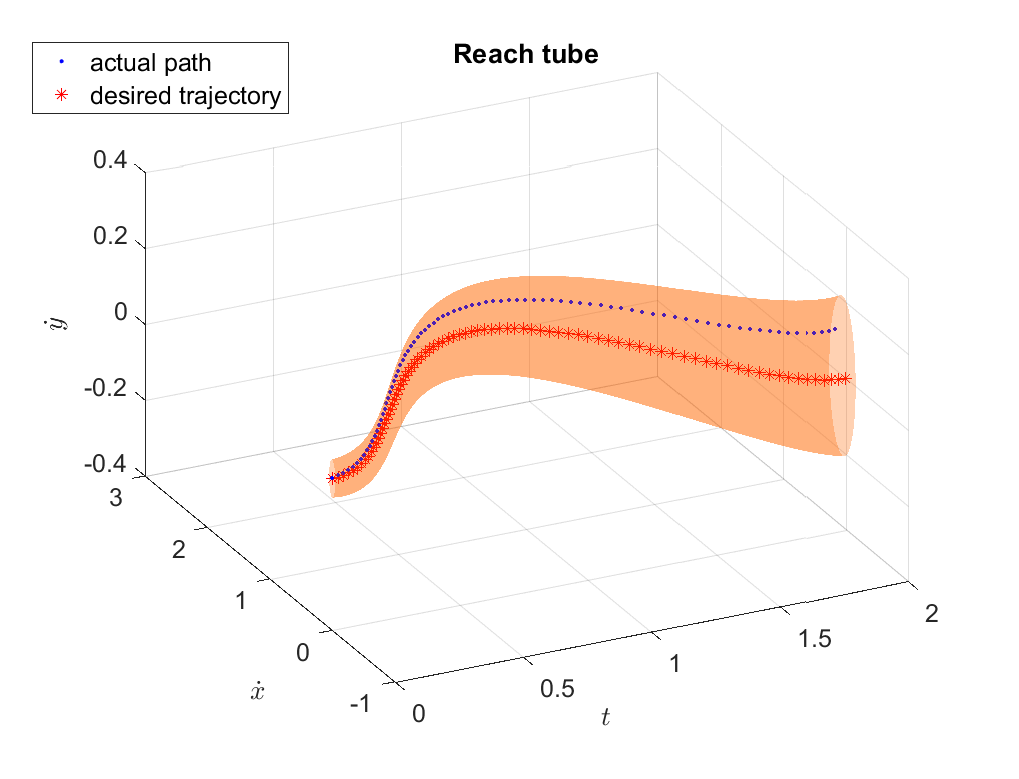
\includegraphics[width = \linewidth ]{fig/reach_set_vel.eps} 
\caption{Velocity Reachable tube for a quadrotor following a straight line trajectory for 2s.}
\vspace{-5pt}
\label{fig:reach_set}\end{wrapfigure}
In this work we propose to research the use of RA to predict reachable states of vehicles under different uncertainties and assess safety constraints like collision avoidance and trajectory tracking. The key idea is that the context (e.g., obstacle configuration) in which the AV is operating dictates the reaction time to switch to a different mode of operation. Thus, predicting as accurately as possible the different situations that can occur in the near future will allow a better safety assessment, \NB{THUS MORE TRUST} and will guide a better planning of actions to perform.
 Let us consider a vehicle modeled generally as a non-linear system of the form $\dot{\bm{x}} = f(\bm{x}, \bm{u}_m)$ with $\bm{x}$ the state vector of the system.
Assume that the system can be linearized around a point $\left(\bm{x}^{*}, \bm{u}^{*}\right)$ (that can be the current operating point) and obtain the following, discretized with sampling time $t_s$, state space representation $\bm{x}(k+1) =  \bm{A} \bm{x}(k) + \bm{B} \bm{u}(k) =  \bm{A} \bm{x}(k) + \bm{B}_m \bm{u}_m(k) + \bm{B}_I f\left(\bm{x}^{*}, \bm{u}^{*}\right) + \bm{B}_d \, \bm{d}$
where $\bm{d}$ is an external disturbance.  %= [d_x \; d_y \; d_z]^{\T}$ is an external disturbance. 
%More details, including a complete mathematical formulation, can be found in \cite{bezzo2016online,bezzo2014cooperative, michael2010grasp, shoukry2015secure, esen17AHS}. 
%}


In this work we propose reachability analysis techniques for safety monitoring AVs and present a machine learning-based approach to minimize runtime computation time.
A reachable set computed at time $t_0$ for a future time $ t_f $ and represented by $R(\bm{x}_0, \bm{u}(t), t_f)$ is an ellipsoid $\epsilon$ that contains all the states $\bm{x}$ reachable at a future time $t_f ~>~ t_0$ where the initial set $ \bm{x}_0 \in \epsilon(\bm{x}_0, \bm{X}_0)$ is bounded by an ellipsoid with center $\bm{x}_0 $ and shape matrix $ \bm{X}_0 $ and the input $ \bm{u}(t) \in \epsilon(\bm{u}(t), \bm{U}) $ is bounded by an ellipsoid with center $ \bm{u}(t) $ and shape matrix $ \bm{U} $. 
%The actual state $\bm{x}(t_f)$ and the estimated state $\tilde{\bm{x}}(t_f)$ will lie inside the reachable ellipsoid. The shape matrix $ \bm{X}_0 $ of the initial state ellipsoid depends on the state uncertainty $ \eta_x $ whereas the shape matrix of the input ellipsoid $ \bm{U} $ depends on the input uncertainty $ \eta_u $. 
A reachable tube $ R(\bm{x}_0, \bm{u}(t), [0,T] ) $ is then defined as the set of all reachable sets over the time interval $\Delta T = [0,T]$, \cite{esen17AHS, VaraiyaEllipsoid2006}. 
The external bound for the reach set at time $ t $ starting from time $t_0 $ is calculated based on the initial state ellipsoid, the plant model, and the input ellipsoid, as follows: 
\vspace{-5pt}
\begin{align*}
R^{+}(t, t_0, \epsilon(\bm{x}_0, \bm{X}_0)) = \bm{\Phi}(t,t_0)\epsilon(\bm{x}_0,\bm{X}_0)
\oplus \int_{t_0}^{t} \bm{\Phi}(t, \zeta) \bm{B}(\zeta) \epsilon(\bm{u}(\zeta), \bm{U})d\zeta
\end{align*}
%\vspace{-5pt}
%\begin{align*}
%R^{+}(t, t_0, \epsilon(\bm{x}_0, \bm{X}_0)) = \bm{\Phi}(t,t_0)\epsilon(\bm{x}_0,\bm{X}_0)
%\oplus \int_{t_0}^{t} \bm{\Phi}(t, \zeta) \bm{B}(\zeta) \epsilon(\bm{u}(\zeta), \bm{U})d\zeta \;\;\;\; \textrm{where}\;\; \bm{\Phi}(t,t_0) = e^{\bm{A}(t-t_0)}
%\end{align*}
where $\bm{\Phi}(t,t_0) = e^{\bm{A}(t-t_0)}$ and $\bm{A}$ and $\bm{B}$ are the state and input matrices related to the AV.
Thus, with this approach, reachable sets can be calculated to capture the uncertain motion of the AV tracking a given trajectory. 
%The set of inputs generated using online simulations, model predictive control, or standard robust control techniques over the interval of time $\Delta t$ can be used to calculate the reachable sets considering that uncertainties may occur at any time during $\Delta t$. 
In Fig.~\ref{fig:reach_set}, the $[\dot x, \dot y]$ velocity reachable tube for an autonomous quadrotor aerial vehicle following a straight line trajectory for 2s \NB{I'll create one for a car}, considering disturbances and measurement and input noise, is shown. 
%\comment{
The blue dotted curve shows the path of the quadrotor whereas the red star curve shows the desired trajectory. The desired trajectory is different from the actual one due to the presence of wind disturbance, however the actual trajectory is contained inside the reachable tubes, since system and sensor uncertainties as well as disturbances are considered when calculating such reachable tubes.
%}
%\begin{wrapfigure}{R}{0.35\linewidth}
%\begin{figure}
%\vspace{-5pt}
%\centering
%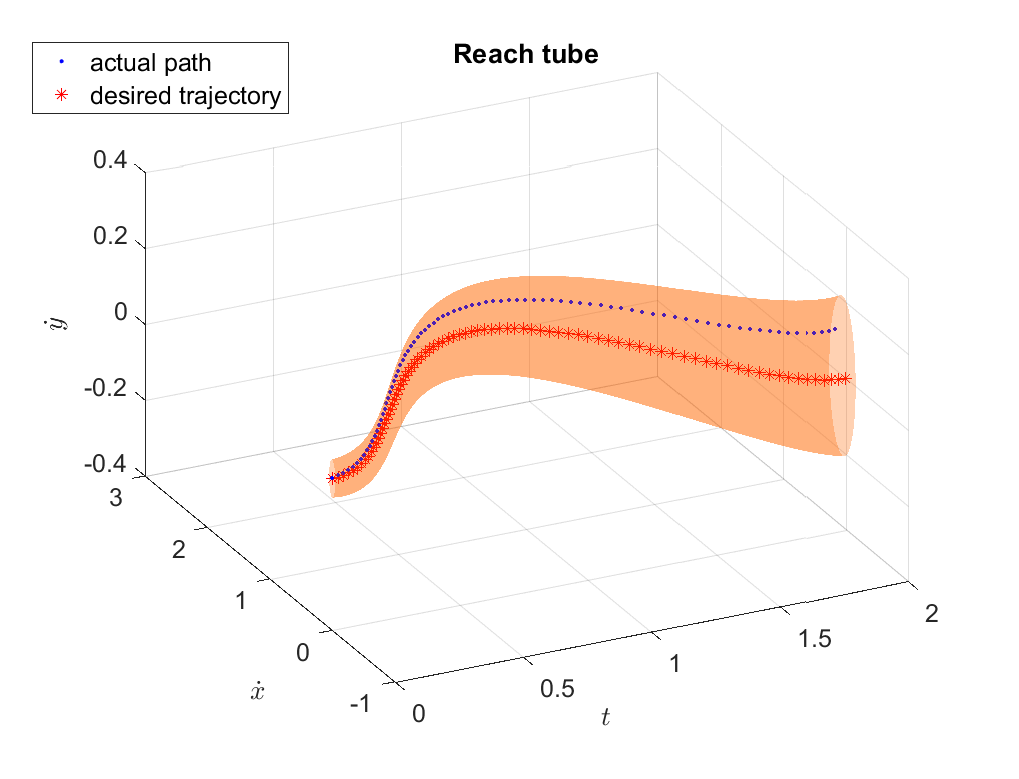
\includegraphics[width = 0.3\linewidth]{fig/reach_set_vel.eps}  %use 0.9
%\caption{Velocity Reachable tube for a quadrotor following a straight line trajectory for 2s.}
%\vspace{-5pt}
%\label{fig:reach_set}
%\end{figure}
%%\end{wrapfigure}

To deal with unmodeled and stochastic system dynamics, we propose a methodology to compute and maximize the probability of maintaining the state of the system within a certain safe region and decide to represent the system as a stochastic hybrid system whose dynamics can be influenced by a control input \cite{abate2007probabilistic, vinod2017forward}. Unlike previous approaches, the safe set can be time-varying \cite{bertsekas1972infinite, bicchi2005control}.
The proposed stochastic reachability methodology is based on formulating the reachability problem as a stochastic optimal control problem. Based on the expression of the probability that the state of the controlled system will evolve within the safe region as a multiplicative cost, dynamic programming (DP) can be used to compute the Markov policy maximizing the cost, and also the maximally safe sets corresponding to different safety levels. 
%\comment{
These are the set of initial conditions for the system, such that there exists a Markov policy capable of maintaining the state of the system within the safe set with a probability greater than a prescribed safety level \cite{tomlin1998synthesizing, balluchi2000maximal,abate2007probabilistic}.
If the objective is to minimize the probability that the system will exit the safe set, then we can formulate the reachability problem as a stochastic optimal control problem, but this time with a cost that is the maximum of a function of the state over the time horizon. Here, again, DP will be considered to determine probabilistic maximal safe sets for Markov policies, \cite{abate2007probabilistic}.
%} 



\noindent\textbf{\em Runtime Verification for Safety-Aware Autonomous Vehicle Operations:} 

% Problem / intro
Offline verification of autonomous vehicles operations may not scale to larger systems where exploring all possible contingencies can be computationally prohibitive. 
For example, an autonomous car can continuously estimating clear roadways and potential obstacles for which the planned trajectory must be verified for safety. To perform offline mission verification would require considering all possible environments (roadways, weather conditions, obstructions, \emph{etc}.).  Moreover, virtually all prior research in the area of formally verifying complex mission planning (expressed using temporal logics) assumes the plan is developed off-line~\cite{saha2014automated,fainekos2005temporal,kress2009temporal}.  However, it is imperative to monitor -- at runtime -- the vehicle to check that the assumptions and properties are indeed satisfied and will continue to hold as the mission evolves. In this thrust, we propose to enable safety-aware learning by performing runtime verification of the control components for mission-critical scenarios where the systems may violate safety constraints.


% Background
 Runtime verification~\cite{SHL12} is a lightweight formal methods technique for online monitoring of evolving traces of observations from a system execution with respect to a formal specification.  Like most other established formal methods, runtime verification techniques target traditional safety-critical systems, developed with respect to specifications, fixed during the system design.  In AVs, it is possible that monitoring specifications will be changing dynamically.  For example, in the presence of external disturbance (like changes in surface type or wind and other atmospheric disturbacnes acting on the vehicle), the system may need to switch mode of operation, reconfigure, adapt its control strategy, and replan its trajectory to fight the disturbance and achieve its desired goal, all while maintaining a certain level of safety assurance. Thus, online prediction for runtime verification is critical to AVs. The main challenge here lies on how to perform runtime monitoring online and efficiently maintaining computation time bounded while guaranteeing system's safety.   To this end, we propose to develop techniques for prediction of autonomous vehicles safety-critical properties (e.g., probability of hitting an obstacle) that can be autonomically verified at runtime.  In this thrust we consider two complementary approaches to runtime verification for safety-aware learning.

 % Proposed work: SMT-based
 Our first approach will be to develop techniques for online verification of missions with AVs. While such problems are computationally very hard, we will leverage our prior work that relies on satisfiability modulo theories (SMT) solvers to address the system of constraints that mix Boolean variables with real variables~\cite{saha2014automated}. One of the major challenges we will address is to verify reactive plans that dynamically compose primitives in order to quickly respond to changes in the environment or mission.  In this approach, our aim is to generate guarantees based on a probabilistic temporal logic framework (such as the framework described in Thrust 1.3) so that we can achieve verified autonomy in unknown environments with learning in the control loop.  Once completed, this will be the first blend of probabilistic formal methods that can reason about probabilistic abstractions of machine learning models in an autonomous system operation.  

% Proposed work: Reachability abstractions
While recent advances in SMT solvers can be leveraged to perform \emph{fast} verification of controllers, the worst-case complexity of such verifications remain troublesome.  This motivates our second approach to runtime verification wherein we abstract the safety conditions such that monitoring can be performed efficiently using predictive techniques (e.g., reachability presented in the previous section). To enable online efficient prediction, hence minimizing computation time and allow real-time monitoring applications, we propose to cast the prediction problem as a two-point boundary value problem (2PBVP) \cite{allen2014machine} and use support vector machine learning algorithms to approximate the reachability boundary using a nonlinear classifier, separating training queries into reachable and non-reachable sets. The idea is to generate training data by solving a large number of 2PBVPs as presented in \cite{allen2014machine} for various randomly generated query pairs. The classifier is then used online to estimate if new query points are reachable. The advantage of such approach is that it can be applied to any system with minimal computation time at runtime since training can be executed offline a priori. \NB{add more discussion here}




\noindent\textbf{\em Safe Reinforcement Learning-based Adaptation:} 

The safety assessment introduced in the previous section is used to guide the AV actions to maintain safety, i.e., to maintain the AV within safe reachable sets. To this end we propose a safe reinforcement learning approach to select appropriate actions for the autonomous system and maintain safety at all the time. The innovation here is that we consider a human in the loop approach in which the desired actions from the user are taken into consideration while determining actions of the AV without violating safety constraints. \NB{need to rephrase but this is the concept we need to convey here} For example, \NB{let's find a proper example here like a user that likes to drive always in the center lane of a highway and is in a rush so it's pushing but there is traffic.}
%Once safety is assessed online, we would like to 
\NB{still working on this section...I'm going to use some of this material but the key idea is to be able to adapt your actions or the AV actions based on how safe the system believes to be} 
Reinforcement Learning (RL) is an area of machine learning concerned with learning how an agent should behave in a given environment in order to maximize some form of cumulative reward. To this end, an agent cycles through a series of transitions which consist of going from one state to the next state by applying actions to the environment and receiving rewards as a consequence of his actions. The goal of RL is to derive a policy, which, given a state, provides the action to take in order to maximize the cumulative reward.
A central problem of RL is thus that of properly assigning the reward to the actions that lead to such reward (a notion known as credit-assignment \cite{kaelbling1996reinforcement, sutton1998reinforcement}). In our case the reward is a combination between user preference and safety \NB{we need to define safety somewhere}
Another main issue of learning behavioral policies in domains that are unknown at first (especially in autonomous vehicles) is that of efficiently bringing the agent from a tabula-rasa state to a condition where the agent is acting as close to optimality as possible. This notion is also known as regret minimization \cite{kaelbling1996reinforcement, sutton1998reinforcement} and is closely related to the topic of trading off exploration of the environment (to sample previously unseen parts of the state-action space) with exploitation of the knowledge accumulated so far. 
An agent that enters the world would therefore need to explore the environment by applying actions and gather data which are as informative as possible so that a policy, encoding the knowledge accumulated so far, is derived. The goal is to go from a situation where the system is mostly exploring the environment to a situation where it is mostly exploiting the accumulated knowledge. 
When the transition probabilities and rewards of a Markov Decision Process (MDP) are known, an agent can obtain the optimal policy without any interaction with the environment. However, exact transition probabilities are difficult for experts to specify and may not be known completely a priori or change over a mission due to aging of the system or unforeseen disturbances and faults. With these considerations in mind, one option left to an agent is a long and potentially costly exploration of the environment. One such algorithm is the E3-algorithm presented in \cite{kearns2002near} in which the basic idea is to repeatedly apply an exploration policy, i.e., one that tries to visit state-action pairs whose transition dynamics are still inaccurately modeled. After a polynomial number of iterations, it will deem itself to have modeled enough of the MDP accurately. Then, it will apply an exploitation policy, which (given the current MDP model) tries to maximize the sum of rewards obtained over time 
. 
In \cite{abbeel2005exploration} the authors demonstrate that the E3-family of algorithms \cite{kearns2002near} is often unacceptable because it requires executing policies that explore also unsafe parts of the workspace, including parts that would lead to a crash of the CPS (e.g. crash of the helicopter discussed in \cite{abbeel2005exploration}). The same authors consider reinforcement learning in systems with unknown dynamics and propose an apprenticeship learning approach, in which an initial teacher demonstration of the task to be learned is presented and then by using only exploitation policies over the training data from the teacher to learn the optimal policy. Farther work from the same authors in \cite{abbeel2006using} deal with scalability issues in reinforcement learning offering a hybrid algorithm that requires only an approximate model and a small number of trials to obtain a near-optimal performance in a real system.
In \cite{epshteyn2008active}, the authors propose another alternative to the suboptimal exploration of the state space presented in the previous works: given initial (possibly inaccurate) specification of the MDP, the agent determines the sensitivity of the optimal policy to changes in transitions and rewards. It then focuses its exploration on the regions of space to which the optimal policy is most sensitive. This technique named Active reinforcement learning enables this type of exploration: it uses sensitivity analysis to determine how the optimal policy in the expert-specified MDP is affected by changes in transition probabilities and rewards of individual actions. This analysis guides the exploration process by forcing the agent to sample the most sensitive actions first. It is shown that the proposed exploration strategy performs well on several control and planning problems.
Reinforcement learning is particularly well-suited to problems with a long-term versus short-term reward trade-off. A key challenge is about enabling online learning while maintain safety.

If the uncertainties of the system's model are high, for example in the event of a failure like a motor outage, then we can think to use a machine learning approach to determine the optimal policy and control inputs to provide to the system to maximize a given reward (e.g. go-to-goal) while learning the new model.
%\begin{wrapfigure}{R}{0.5\linewidth}
%\vspace{0em} 
%\centering
%  \includegraphics[width = \linewidth]{figures/RL.png}
%%  \vspace{-18pt} 
%\caption{The proposed reinforcement learning approach for prediction augmented with the update loop to consider unmodeled efefcts from disturbance, noise, and other unpredicted adversarial effects.}
%%\vspace{-10pt}
%\label{fig:rl}\end{wrapfigure}
More specifically in this task we propose an iterative reinforcement learning (RL) framework to determine the control policy and refine the model of the system. The abstract setting can be described in the following terms: a AV is assumed to act according to an optimal policy for a Markov decision process $M^{\mbox{S}}$. The system knows its current state and action sets as well as the initial transition probabilities for $M^{\mbox{S}}$. Due to unforeseen disturbances and unpredicted behaviors (e.g., environmental disturbances, high traffic) the transition probability model changes, but the reward function remains the same. The model is not completely known and need to be refined as the system is running. This problem can be cast as an MDP problem in which transition probabilities are changed and adapted at every iteration to handle unknown environments and systems dynamics. Current and historic measurements and inputs will be used to refine the current model and update transition probabilities. We can think to leverage reachability analysis also in this task to incorporate uncertainties as the RL-based approach converges to a model and policy and to predict accordingly the possible future states that the vehicle may cover. 
%As the model get refined and updated we can then think to consider reachability analysis to predict future states of the system including incorporating uncertainties in the model \NB{cite here}


\NB{I may remove the following section} An even reacher extension to this planned work will consider disturbance and uncertainties in the model and environmental dynamics as an adversarial player with an unknown reward that we would like to learn. This specific problem can be solved with a number of inverse reinforcement learning algorithms. 
For this case we can still model the decision problem as an MDP $M^{\mbox{D}}$ in which reward is structured around misclassification cost experienced in terminal states that correspond either to allowing the AV to proceed to its intended terminal state or to change control law. The state definition for $M^{\mbox{D}}$ includes all of the vehicle state elements as well as a belief function for the vehcile reward function.
Because it includes a belief state, MDP will generally suffer from the curse of dimensionality and be intractable from the perspective of full-width planning methods.  To address this issue, we propose to make use of  work on Monte-Carlo planning in large partially-observed MDPs (POMDPs) \cite{silver2010monte}.  The basic idea is to use a simulator as a generative model of the decision process.  The simulator is used to generate sequences of states, observations, and rewards that are used to update the value function.  
%A key feature of the approach is that explicit representation of model dynamics is not needed.  In our case, this means that we can use a simulator in which the next observed action on the part of the subject (along with previous observations) is used in a Bayesian IRL procedure to find the new belief state for reward. 
Following \cite{silver2010monte} and others, sampling will be done according to a Monte-Carlo trees search algorithm.  Other methods, such as DESPOT  \cite{somani2013despot}, and  recent POMDP computational methods \cite{baier2012nested,guez2012efficient,guez2013scalable,vien2013monte}  will also be considered.


\noindent\textbf{Correct-by-construction controller synthesis}

In co-PI Feng's prior work~\cite{feng2015controller,feng2016synthesis}, we proposed a stochastic game based approach to automatically synthesize correct-by-construction control protocols (mission plans) for an unmanned aerial vehicle (UAV) while accounting for the uncertainty of human operators. By modeling the UAV as a player and the human operator as another player in the stochastic game, we reduced the problem to finding a winning strategy for the UAV against all strategies (including the worst-case) of the human operator. The synthesized UAV control protocol is guaranteed to satisfy the mission objectives (expressed as temporal logic specifications) imposed on the stochastic game. Furthermore, using different human operator models, our approach enables the synthesis of operator-dependent optimal mission plans for the UAV, highlighting the effects of operator characteristics (e.g., workload, proficiency, and fatigue) on the mission performance. The proposed research will build on our prior work and develop new methods for synthesizing control protocols for autonomous vehicles while accounting for the behavior models leanred in Thrust I. We will propose an approach build upon techniques of strategy synthesis from stochastic multi-player games~\cite{SK16}, which often involve the computation of winning strategies based on value iteration algorithms. 
We will take into account cognitive mechanism and develop new techniques for the automated synthesis from the logic PRTL*. 
In addition, we will consider multi-objective properties that require simultaneous satisfaction of multiple safety and trust properties.
For example, ``agent $A$ (human)'s trust in agent $B$ (autonomous vehicle)'s capabilities to keep a safe distance with the front vehicle is at least 80\%'' \emph{and} ``the vehicle should maintain a minimal speed of 60 mph on the highway''.
We will develop techniques that compute an $\varepsilon$-approximation of the Pareto set of optimal trade-offs between the individual properties.
The synthesized strategies can inform the design of autonomous vehicles, e.g., what actions should the vehicle take in order to gain human trust?
   